\clearpage
\part{Hangman}

In this part, you will implement a version of the ``terminal hacking'' minigame from \emph{Fallout~4} (Bethesda, 2015).
In this minigame you must guess a hidden $n$-letter word, one of several options presented to you.
On choosing an option, you are told the \emph{likeness}: the number of letters which match the hidden word (i.e.\ the same letter in the same position).
For example if the hidden word is \texttt{HOUSE} and your guess is \texttt{MOUSE}, the likeness is $4$ out of $5$.
If your guess is \texttt{HOPES}, the likeness is $2$ out of $5$ (the letters \texttt{S} and \texttt{E} do not count as they are in the wrong position).

The provided skeleton project contains code for reading a list of words from a text file, and choosing the words at random.
You will implement the rest of the game.

\section{} \label{core-a-first}

The following algorithm takes a guessed word and the secret word, and returns the number of letters which match according to the game rules.

\begin{algorithm}
\begin{algorithmic}
    \Procedure{GetLikeness}{guessedWord, secretWord}
        \State $\text{result} \gets 0$
        \For{$i = 0, 1, \dots, \text{secretWord.length} - 1$}
            \If{$\text{secretWord}[i] = \text{guessedWord}[i]$}
                \State increment result
            \EndIf
        \EndFor
        \State \textbf{return} result
    \EndProcedure
\end{algorithmic}
\end{algorithm}

\textbf{Implement} the algorithm as a C++ function, choosing appropriate data types for the parameters, return value, and any variables.

\section{}



\section{} \label{core-a-last}

\textbf{Implement} a playable Hangman game, using the functions implemented above and structured
according to the following flowchart:

\begin{center}
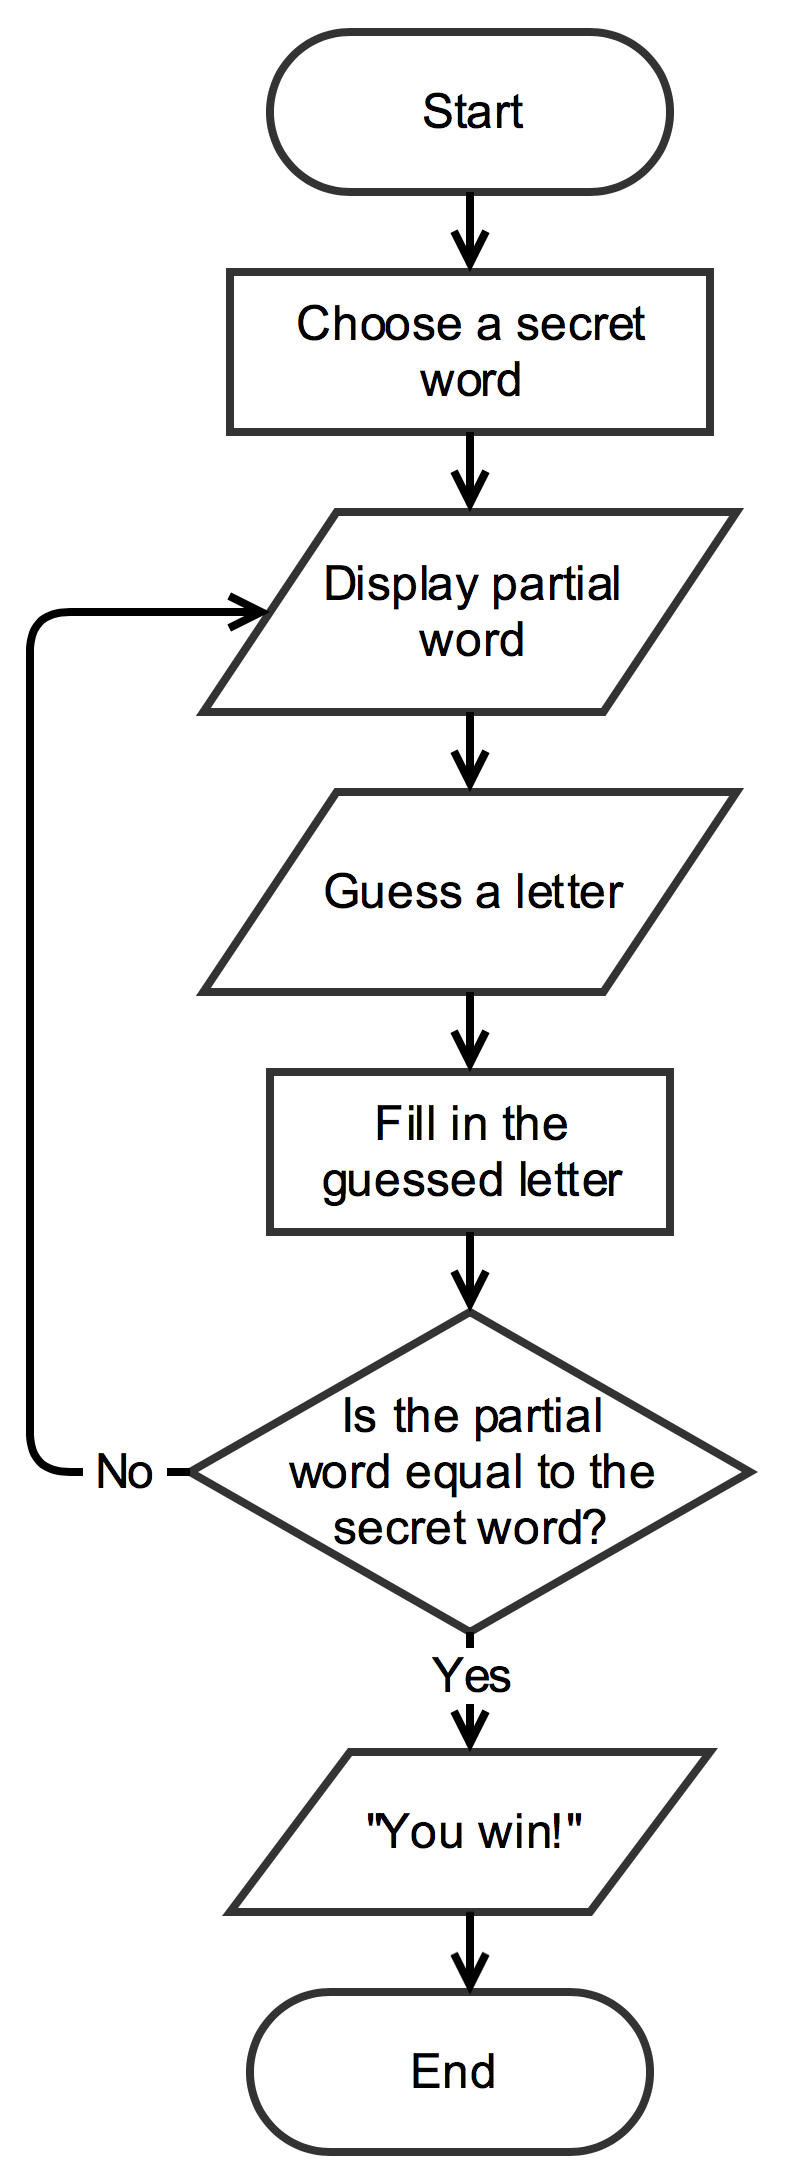
\includegraphics[height=0.5\textheight]{hangman_flowchart.png}
\end{center}

\section{Stretch goal} \label{stretch-a}

The game would be more interesting if the player had a limited number of lives in which to guess the word,
and lost a life for guessing a letter which was not present in the word.

\textbf{Modify} the flowchart above to make this change. \textbf{Modify} your C++ program to reflect your revised flowchart.
